\documentclass[12pt,a4paper]{report}

\usepackage[utf8]{vietnam}

\usepackage {graphicx}

\usepackage{amsmath, amsthm, amssymb,latexsym,amscd,amsfonts,enumerate}

\usepackage[top=3.5cm, bottom=3.0cm, left=3.5cm, right=2.0cm]{geometry} % căn lề theo quy chuẩn KLTN

\usepackage{color, fancyhdr, graphicx}
\usepackage{wrapfig}
\usepackage[unicode]{hyperref}



%\pagenumbering{roman}\pagestyle{plain}

\pagestyle{fancy}

\lhead{\it \color{blue}{BTL Nhập môn điện toán }}

\rhead{\it \color{blue}{Trường Đại học Bách Khoa Tp HCM}}

\lfoot{\it \color{blue}{Nhóm 1}}

\rfoot{\it  \color{blue}{Khoa KHKT Máy tính năm 2018-2019}}

\renewcommand{\headrulewidth}{1,2pt}

\renewcommand{\footrulewidth}{1,2pt} % Cái này là tiêu đề chạy
\pagenumbering{arabic}

\begin{document}

\fontsize{13pt}{18pt}\selectfont % Lệnh thay đổi cỡ chữ thành cỡ 13, cỡ dòng 18 (theo quy chuẩn của Khóa Luận TN).

\setlength{\baselineskip}{18truept}

\begin{titlepage} % Đây là trang bìa

\begin{center}

{\large\bf TRƯỜNG ĐẠI HỌC BÁCH KHOA }\\
{\large\bf ĐẠI HỌC QUỐC GIA }\\
{\large\bf THÀNH PHỐ HỒ CHÍ MINH }\\

{———————o0o——————–}

\vskip 1cm



	
\includegraphics[width=0.3\linewidth]{logg}

	\label{fig:logg}


\vskip 1cm

{\Large\bf \textbf{\color{blue}{BÁO CÁO BÀI TẬP LỚN NHẬP MÔN ĐIỆN TOÁN}}}\\

\vskip 1cm

{\bf {\it \color{blue}{Nhóm:}} \color{blue}{NHÓM 1 }} \hspace{0.5cm} {\bf {\it \color{blue}{Lớp:}} \color{blue}{L10}}

\vskip 3cm

\begin{tabular}{r l}

Giảng viên hướng dẫn:&{\bf QUẢN THÀNH THƠ }\\ &{\bf PHẠM TRUNG KIÊN}\\
[0.5cm]

Sinh viên:&{\bf NGUYỄN NGỌC TÂN - 1813942}\\
Sinh viên:&{\bf NGUYỄN LƯƠNG HOÀI SƠN - 1813854}\\
Sinh viên:&{\bf NGUYỄN VĂN QUÝ - 1813760}\\
Sinh viên:&{\bf NGUYỄN PHẠM ANH TÀI - 1813897}\\
[0.5cm]



\end{tabular}

\vfill

{\bf TP HỒ CHÍ MINH, 16/12/2018}

\end{center}

\end{titlepage}

\chapter{Lời nói đầu}
{\bf Đặt vấn đề}\vskip 0.4cm
+ Vấn đề khi làm việc cá nhân: bạn đang làm việc với một số tập tin và thư mục nào đó (gọi đơn giản là file). Hàng ngày, bạn tiến hành nhiều thay đổi trên các file này. Vào một ngày xấu trời nào đó, bạn cần quay lại thời điểm của những file này cách đây 2 ngày thì bạn phải làm sao?\vskip 0.4cm

+ Vấn đề khi làm việc nhóm: bạn và vài người bạn của bạn đang làm việc trên một số file (hay project), làm sao để nhiều người làm việc hiệu quả trên các file này (không có những trường hợp ghi đè nội dung của nhau, xóa nhầm file, quản lý được ai thao tác trên các file nào... )\vskip 0.4cm

Từ hai vấn đề trên các thành viên trong nhóm đã tìm hiểu trên nhiều nguồn tài liệu và biết đến công cụ quản lí mã nguồn có thể giải quyết được các vấn đề trên và hơn thế nữa. Sau khi có được chủ đề bài tập lớn, nhóm đã cùng nhau tìm hiểu về Git - một công cụ quản lý mã nguồn rất phổ biến. Sau thời gian học tập và tìm kiếm tài liệu trên mạng, thông qua quá trình thực hành nhóm đã có những kiến thức cơ bản nhất. Và dưới đây chính là những kiến thức mà nhóm đã tìm hiểu được về Git.


\tableofcontents % Lệnh mục lục

\chapter{Giới thiệu VCS} % Chương 1

%\addcontentsline{toc}{chapter}{{\bf Giới thiệu VCS}\rm} 

\hspace{0.6cm} •	Hệ thống quản lý phiên bản (VCS) là một hệ thống ghi lại những thay đổi trên một tệp hay tập hợp các tệp theo thời gian để mà chúng ta có thể khôi phục lại các phiên bản trước.
\vskip 0.4cm
•	VCS cho phép chúng ta \\
- Khôi phục lại phiên bản cũ của tệp hay cả dự án\\
- Xem lại các thay đổi được thực hiện theo thời gian\\
- Quan sát xem ai người gây ra vấn đề và còn nhiều thứ khác\vskip 0.4cm
•	Có 3 loại quản lý phiên bản: Hệ thống quản lý phiên bản cục bộ (Local Version Control Systems), tập trung (Centralized Version Control Systems) và phân tán (Distributed Version Control Systems). Dưới đây chúng ta tập trung vào hệ thống quản lý phiên bản phân tán (DVSC), cụ thể là Git.\\

\chapter{Giới thiệu GIT}

%\addcontentsline{toc}{chapter}{{\bf Giới thiệu GIT}\rm} 

\section{Lịch sử}

%\addcontentsline{toc}{chapter}{{\bf Lịch sử}\rm} 

\hspace{0.6cm}- Năm 2002, dự án Linux kernel bắt đầu sử dụng một hệ thống quản lý phiên bản phân tán (DVSC) có bản quyền là BitKeeper. \vskip 0.4cm
- Năm 2005, mối quan hệ giữa cộng đồng phát triển Linux kernel và công ty thương mại đã phát triển BitKeeper đổ vỡ.  \vskip 0.4cm
- Điều đó thúc đẩy cộng đồng phát triển Linux tạo ra một công cụ của riêng họ, dựa trên những điều học được khi sử dụng BitKeeper. \vskip 0.4cm

\section{Tổng quan về Git}

%\addcontentsline{toc}{chapter}{{\bf Lời nói đầu}\rm} 

\hspace{0.6cm}•	Cách xử lý dữ liệu:\vskip 0.4cm
- Git coi dữ liệu của nó là một tập các ảnh (snapshot) của hệ thống tập tin. Điều này có nghĩa là mỗi phiên bản của dự án (có thể hiểu là một commit) sẽ là tập hợp của một số ảnh lưu (snapshots) lại nội dung của các tập tin của phiên bản đó.\vskip 0.4cm
- Điều này mang đến nhiều tiện lợi cho việc theo dõi lịch sử, phục hồi dữ liệu. \vskip 0.4cm
•	Thao tác với dữ liệu:\vskip 0.4cm
- Hầu hết các thao tác với dữ liệu của Git có thể thực hiện cục bộ. Git thực hiện được việc này vì toàn bộ dữ liệu của dự án đều được lấy về và lưu trữ trên máy tính của người dùng.\vskip 0.4cm
- Với tính năng này của Git, người dùng có thể làm việc trong nhiều trường hợp mà không nhất thiết phải có kết nối Internet. Điều này mang đến nhiều lợi thế cho Git so với các hệ thống quản lý dữ liệu khác.\vskip 0.4cm
•	Tính toàn vẹn:\vskip 0.4cm
- Các thay đổi trong Git được tham chiếu bằng một mã băm sử dụng cơ chế mã hóa SHA-1. Đồng thời, các thay đổi trong Git đều được thêm vào cơ sở dữ liệu do đó rất khó bị mất khi thay đổi và truyền tải dữ liệu. Với Git, người dùng có thể thoải mái thử nghiệm, lưu trữ mà không sợ ảnh hưởng đến dự án.\vskip 0.4cm

Tổ chức dữ liệu trong Git: các tập tin trong Git tồn tại ở một trong ba trạng thái là modified, staged và committed.\vskip 0.4cm
•	{\it Modified}: tập tin được sửa nhưng chưa được đánh dấu để commit (nằm trong mục Unstaged files).\vskip 0.4cm
•{\it	Staged}: tập tin được đánh dấu sẽ được commit (nằm trong mục Staged files).\vskip 0.4cm
•{\it	Committed}: tập tin đã được commit và lưu trữ trong cơ sở dữ liệu.\vskip 0.4cm
(Một tập tin có thể vừa ở trạng thái modified vừa ở trạng thái staged hoặc committed. Điều này xảy ra khi người dùng chỉ staged một số dòng trong tập tin.)\vskip 0.4cm
Ba trạng thái này tạo ra ba phần riêng biệt của dự án:\vskip 0.4cm
•{\it	Working directory}: là bản sao của một phiên bản của dự án. Người dùng sẽ làm việc với các tập tin ở khu vực này. Mọi thay đổi của các tập tin sẽ được hiển thị ở đây.\vskip 0.4cm
•	{\it Staging area}: là một tập tin trong thư mục Git. Tập tin này chứa thông tin về những thay đổi sẽ được commit.\vskip 0.4cm
•{\it	Git directory}: đây là nơi Git lưu trữ các siêu dữ liệu (metadata) và cơ sở dữ liệu của toàn bộ dự án. Đây cũng là phần quan trọng nhất của Git, nó là một bản sao của dự án được sao chép (clone) từ repository trên server Git.\vskip 0.4cm

\newpage
\section{Download và cài đặt}

%\addcontentsline{toc}{chapter}{{\bf Download và cài đặt}\rm} 

\hspace{0.6cm}- Link download: {\it https://git-scm.com/downloads \vskip 0.4cm}
- Git hỗ trợ các nền tảng Windows, MacOS, Linux/UNIX\vskip 0.4cm
- Hiện tại là phiên bản 2.19.2\vskip 0.4cm


\newpage % Mấy lệnh \newpage và abc, xyz này khi gõ thì các bạn bỏ đi nhé!





\chapter{Cách sử dụng} 


\section{Thiết lập ban đầu} 
\hspace{0.6cm}{\bf a. Git folder structure ( Cấu trúc thư mục Git)}\vskip 0.4cm
- Git có một công cụ có sẵn gọi là \textbf{git config}, cho phép ta xem và điều chỉnh các biến cấu hình để điều khiển được mọi khía cạnh của Git \vskip 0.4cm
{\bf b. Danh tính của người dùng}\vskip 0.4cm
- Điều đầu tiên bạn nên làm sau khi cài đặt Git đó là đặt tên người dùng và địa chỉ email của bạn.\vskip 0.4cm
- Điều này quan trọng bởi vì mỗi commit trong Git đều sử dụng thông tin này, những thông tin này sẽ mãi gắn với các commit.\vskip 0.4cm
- Hai thông tin này phải được cái đặt trước khi thực hiện mọi thao tác trên Git vì khi bạn ủy thác thông tin lên Git thì Git sẽ phân biệt và nhận dạng thông qua username và useremail\vskip 0.4cm
+ Để đặt tên người dùng, ta dùng lệnh: {\it  git config \texttt{-{}-}global user.name “Your name”} \vskip 0.4cm
+ Để đặt email: {\it git config \texttt{-{}-}global user.email john@example.com}\vskip 0.4cm
%\begin{figure}
	%\centering
	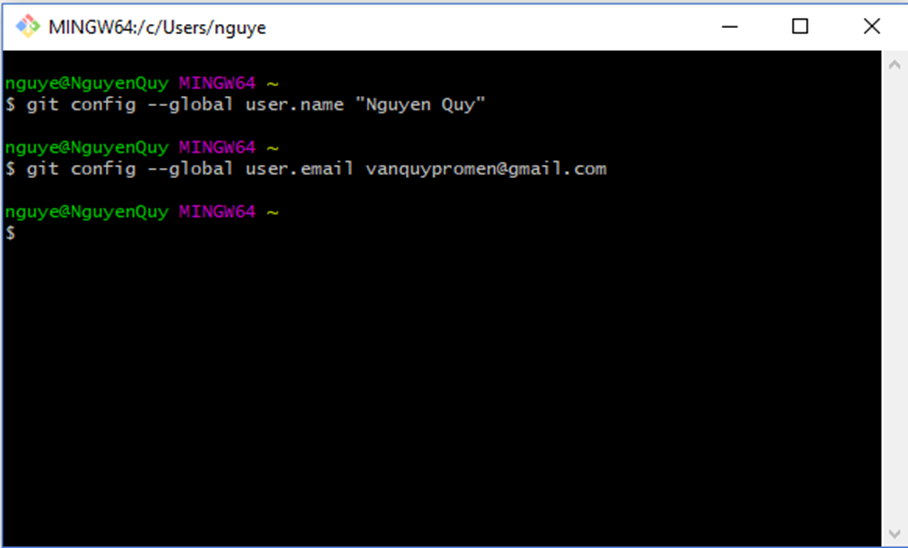
\includegraphics[width=0.8\linewidth]{screenshot001}
%	\caption{}
	\label{fig:screenshot001}
%\end{figure}
\vskip 0.4cm
\vskip 0.4cm
{\bf c. Trình soạn thảo}\vskip 0.4cm
- Ở bước cài đặt Git, chúng ta đã chọn Visual Studio Code làm công cụ chỉnh sửa mặc định\vskip 0.4cm
- Nếu muốn thay đổi công cụ mặc định đã được cài đặt trước đó thì có thể sử dụng lệnh:\vskip 0.4cm
{\it git config \texttt{-{}-}global core.editor “ ’[đường dẫn đến công cụ trong máy bạn]’ -multilnst -nosession”}\vskip 0.4cm
Ví dụ: muốn cho Visual Studio Code làm công cụ soạn thảo mặc định cho Git\vskip 0.4cm
\vskip 0.4cm
	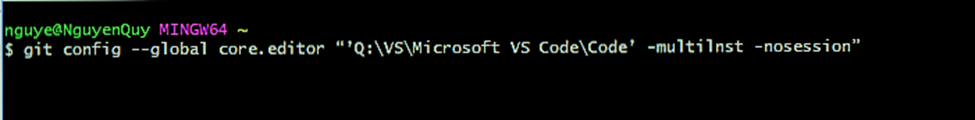
\includegraphics[width=0.8\linewidth]{screenshot002}
	%\caption{}
	\label{fig:screenshot002}
\vskip 0.4cm \vskip 0.4cm
{\bf d. Kiểm tra các cài đặt} \vskip 0.4cm
- Khi muốn kiểm tra các cài đặt, ta dùng lệnh git config \texttt{-{}-}list. Kết quả như hình bên dưới: 
\vskip 0.4cm
	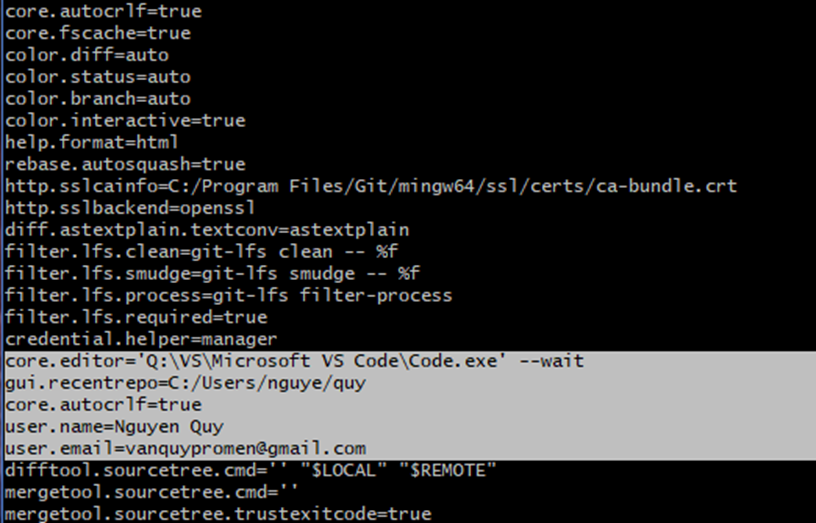
\includegraphics[width=0.8\linewidth]{screenshot003}
	\label{fig:screenshot003}\vskip 0.4cm\vskip 0.4cm

- Ta có thể kiểm tra giá trị của từng khoá riêng biệt bằng lệnh: {\it git config \{khoá\}}\vskip 0.4cm
- Ví dụ như ta muốn xem tên người dùng và địa chỉ email, ta gõ lệnh như trong hình: \vskip 0.4cm

	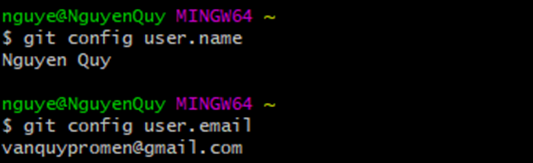
\includegraphics[width=0.8\linewidth]{screenshot004}
%	\caption{}
	\label{fig:screenshot004}
%\end{figure}
 \vskip 0.4cm\vskip 0.4cm
{\bf e. Giúp đỡ} \vskip 0.4cm
 - Có ba cách để hiển thị trang hướng dẫn cho các lệnh trong Git \vskip 0.4cm
 + git help <lệnh> \vskip 0.4cm
 + git <lệnh> \texttt{-{}-}help \vskip 0.4cm
 + man git-<lệnh>  \vskip 0.4cm
 




\section{Khởi tạo Repository}
\hspace{0.6cm}{\bf a. Khởi tạo một repository trong một thư mục có sẵn} \vskip 0.4cm
- Repository, hay còn gọi là Repo, trong tiếng Việt nghĩa là kho chứa. Repo là nơi chứa tất cả mã nguồn cho một dự án được quản lý bởi Git.\vskip 0.4cm
- Nếu bạn muốn bắt đầu quản lý một dự án có sẵn bằng Git, bạn cần di chuyển đến thư mục đó sử dụng bash và gõ: \textit{git init}\vskip 0.4cm
- Để di chuyển đến thư mục, ta sử dụng lệnh: {\it cd <đường dẫn thư mục> }\vskip 0.4cm

	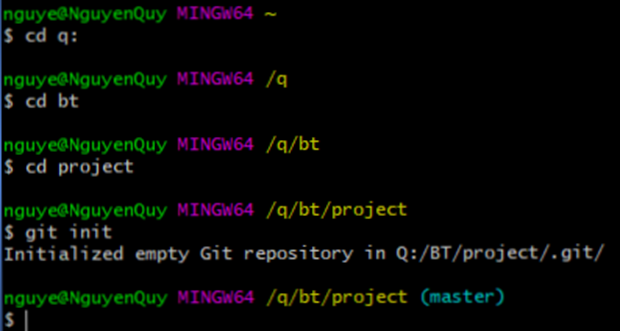
\includegraphics[width=0.8\linewidth]{screenshot005}

	\label{fig:screenshot005}
\vskip 0.4cm\vskip 0.4cm

- Ở hình trên, sử dụng lệnh cd để di chuyển đến thư mục project chứa bài tập lớn cần quản lý có đường dẫn là {\it Q:/BT/project} và sau đó sử lệnh {\it git init} để tạo ra một thư mục tên là .git, thư mục này chính bộ khung xương của Repo.\vskip 0.4cm
{\bf b. Sao chép một Repo có sẵn} \vskip 0.4cm
- Nếu bạn muốn có một bản sao của một Git repo có sẵn, ví dụ như repo của một dự án mà bạn muốn tham gia, sử dụng lệnh {\it git clone <đường dẫn đến repo>}\vskip 0.4cm
- Đường dẫn có thể là link dẫn đến kho lưu trữ mã nguồn của nhóm làm việc với bạn trên nền web như GitHub\vskip 0.4cm

\section{Quản lý Repository}

\hspace{0.6cm}{\bf a. Vòng tuần hoàn trạng thái của tệp}\vskip 0.4cm

	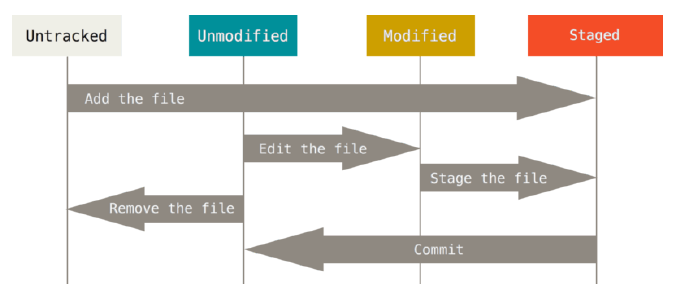
\includegraphics[width=0.8\linewidth]{screenshot006}
	
	\label{fig:screenshot006}
\vskip 0.4cm\vskip 0.4cm
- Untracked: tệp chưa được theo dõi (track)\vskip 0.4cm
- Unmodified: tệp đã được commit\vskip 0.4cm
- Modified: tệp đã được chỉnh sửa và chưa commit\vskip 0.4cm
- Staged: các tệp đã được theo dõi hoặc các tệp đã chỉnh sửa đang chờ để commit\vskip 0.4cm
{\bf b. Kiểm tra trạng thái của tệp} \vskip 0.4cm
- Lệnh \textit{git status} dùng để kiểm tra trạng thái của thư mục đang làm việc hiện tại.\vskip 0.4cm
+ Dưới đây, ta kiểm tra trạng thái của thư mục làm việc (working directory) hiện tại là project\vskip 0.4cm

	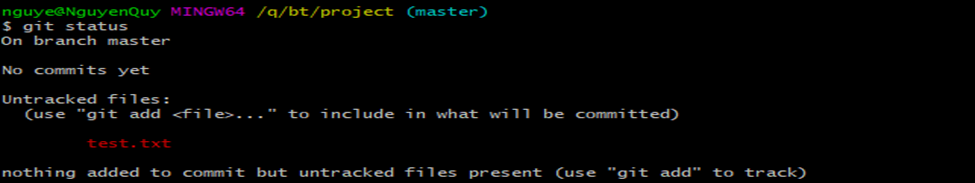
\includegraphics[width=0.8\linewidth]{screenshot007}

	\label{fig:screenshot007}
\vskip 0.4cm\vskip 0.4cm
Ở hình trên, ta thấy tệp test.txt không được thêm vào Repo, đang ở trạng thái untracked (chưa được theo dõi)\vskip 0.4cm
- Để theo dõi một tập tin, ta dùng lệnh {\it git add <tên tệp>}, cụ thể ở đây ta theo dõi tệp test.txt\vskip 0.4cm

	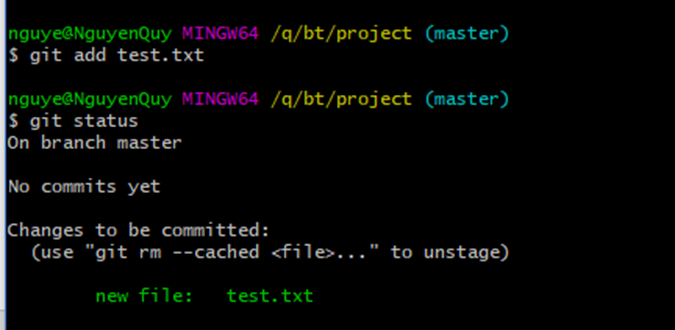
\includegraphics[width=0.8\linewidth]{screenshot008}

	\label{fig:screenshot008}
\vskip 0.4cm\vskip 0.4cm
{\bf c. Bỏ qua các tập tin} \vskip 0.4cm
- Tệp .gitignore liệt kê những file mà mình không mong muốn cho vào Git (Git sẽ lờ những file đó đi)\vskip 0.4cm
- Tạo file gitignore bằng lệnh touch .gitignore\vskip 0.4cm
- Các pattern format hay dùng:\vskip 0.4cm
•	Sử dụng \# để comment và có thể để cách dòng cho dễ đọc.\vskip 0.4cm
•	Đơn giản nhất là tên file cần ignore: example.exe, example.txt, …\vskip 0.4cm
•	Hay cả thư mục: example\_folder/\vskip 0.4cm
•	Sử dụng * để tìm các file có cùng định dạng. Ví dụ như bạn muốn Git bỏ qua tất cả các file .xml trong project: *.xml\vskip 0.4cm
Ví dụ: \vskip 0.4cm
- Trong Repo hiện tại có thư mục bin và ta muốn Git bỏ qua thư mục đó\vskip 0.4cm

	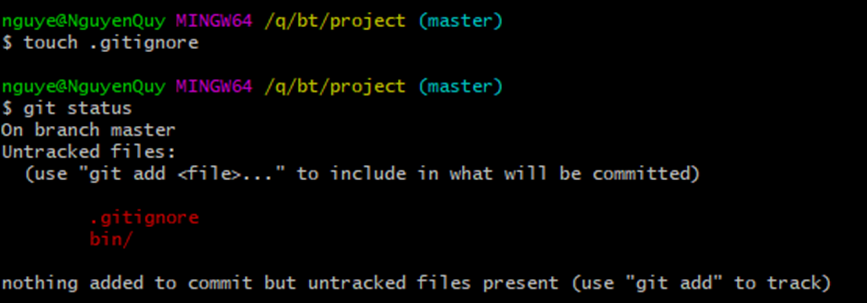
\includegraphics[width=0.8\linewidth]{screenshot009}

	\label{fig:screenshot009}
\vskip 0.4cm\vskip 0.4cm
- Ta chỉnh sửa file .gitignore để thêm thư mục bin vào\vskip 0.4cm

	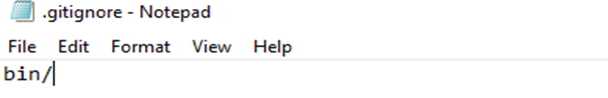
\includegraphics[width=0.8\linewidth]{screenshot010}
	
	\label{fig:screenshot010}
\vskip 0.4cm\vskip 0.4cm
- Sau khi thêm bin vào .gitignore, ta kiếm tra lại trạng thái và thấy thư mục bin đã bị Git bỏ qua.
\vskip 0.4cm
	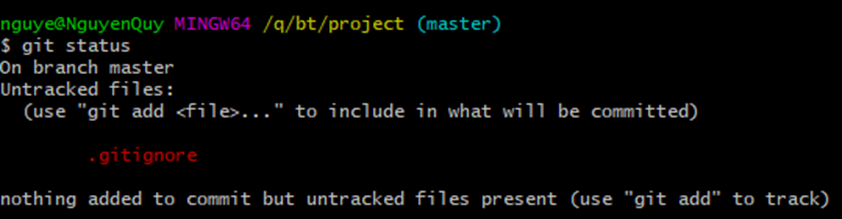
\includegraphics[width=0.8\linewidth]{screenshot011}

	\label{fig:screenshot011}
\vskip 0.4cm\vskip 0.4cm
{\bf d. Xem các thay đổi} \vskip 0.4cm
- Câu lệnh {\it git status} vẫn còn mơ hồ, ta không thể biết chính xác được cái gì đã được thay đổi\vskip 0.4cm
- Lệnh {\it git diff} cho ta biết chính xác từng dòng được thêm vào hay xoá đi\vskip 0.4cm
- Câu lệnh {\it git diff \texttt{-{}-}staged} đã được tổ chức (staged) và chuẩn bị được commit.\vskip 0.4cm
{\bf e. Commit các thay đổi}\vskip 0.4cm
- Sau khi đã tổ chức các tập tin theo ý muốn, chúng ta có thể commit chúng\vskip 0.4cm
- Lưu ý rằng những thứ chưa được tổ chức (unstaged) – những file được tạo ra hoặc chỉnh sửa sau khi bạn chạy lệnh \textit{git add} sẽ không được commit, do những file vẫn đang ở trạng thái modified.\vskip 0.4cm
- Cách đơn giản để commit đó là dùng lệnh: {\it git commit –m “message”}\vskip 0.4cm
+ Sau khi đã đưa các tệp lên trạng thái staged ta phải sử dụng lệnh: {\it git commit -m “initial project version”} (initial project version chính là message, tóm tắt nội dung của lần commit này) để commit các tệp đang ở trạng thái staged\vskip 0.4cm

	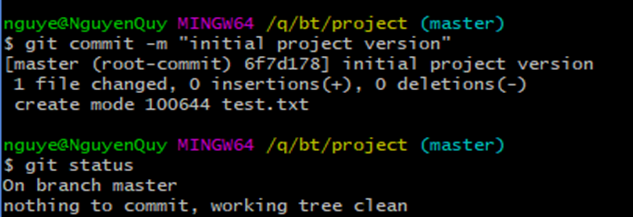
\includegraphics[width=0.8\linewidth]{screenshot012}

	\label{fig:screenshot012}
\vskip 0.4cm\vskip 0.4cm
+ Kết quả ta sẽ được như hình trên, tệp test.txt đã được commit.\vskip 0.4cm
{\bf f. Bỏ qua khu vực tổ chức (staging area)}\vskip 0.4cm
- Thêm lựa chọn -a vào câu lệnh git commit sẽ làm Git tự động tổ chức (stage) tất cả những tệp đã được theo dõi trước khi thực hiện commit, cho phép ta bỏ qua bước \textit{git add}\vskip 0.4cm
- Có thế add hết tất cả các tệp untracked vào staged bằng lệnh: {\it git add \texttt{-{}-}all}\vskip 0.4cm

	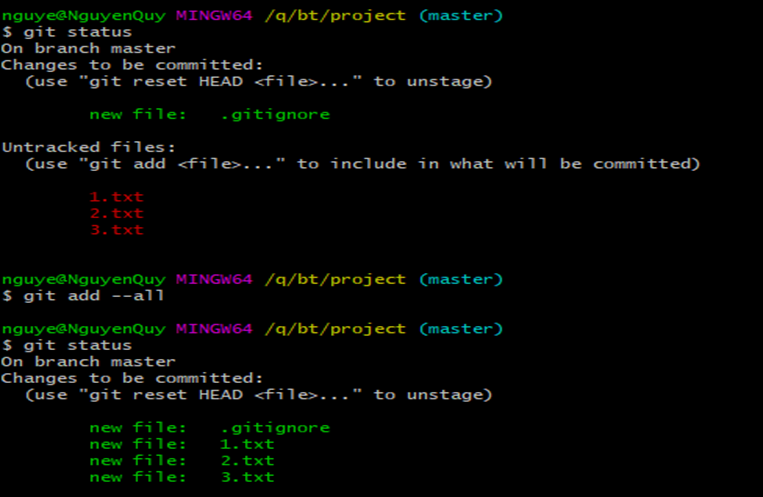
\includegraphics[width=0.8\linewidth]{screenshot013}

	\label{fig:screenshot013}
\vskip 0.4cm\vskip 0.4cm
- Ở hình trên, có 3 tệp untracked, sử dụng {\it git add \texttt{-{}-}all} để đưa cả 3 tệp vào stage area cùng lúc\vskip 0.4cm
- Sau đó commit 1 lần 3 tệp trên bằng lệnh {\it git commit –a –m “commit flie”}, kết quả sẽ được như hình dưới\vskip 0.4cm

	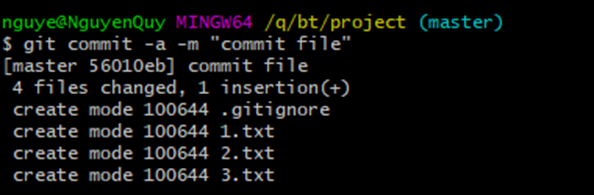
\includegraphics[width=0.8\linewidth]{screenshot014}

	\label{fig:screenshot014}\vskip 0.4cm\vskip 0.4cm

{\bf g. Xoá tập tin} \vskip 0.4cm
- {\it git rm}: Xoá một tập tin khỏi staging area, đồng thời cũng xoá tập tin đó trên ổ cứng.\vskip 0.4cm
- {\it git rm \texttt{-{}-}cached} : tập tin không còn bị kiếm soát bởi Git nhưng mà vẫn còn trên ổ cứng\vskip 0.4cm


	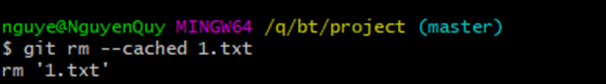
\includegraphics[width=0.8\linewidth]{screenshot015}
	
	\label{fig:screenshot015}
\vskip 0.4cm\vskip 0.4cm
{\bf h. Di chuyển tập tin}
- Để đổi tên một tập tin trong Git, ta dùng lệnh sau: {\it git mv file\_from file\_to}\vskip 0.4cm

	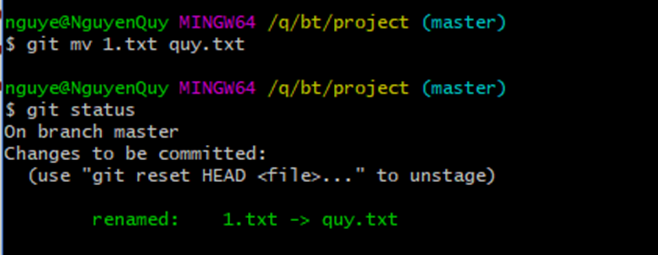
\includegraphics[width=0.8\linewidth]{screenshot016}

	\label{fig:screenshot016}




	\newpage
\section{Xem lịch sử commit}
\hspace{0.6cm}- Áp dụng khi xem lại các dòng code, các đoạn commit có sai sót gì, kiểm tra các đoạn chỉnh sửa những gì\vskip 0.4cm
- Công cụ đơn giản và tốt nhất để thực hiện việc này là lệnh: {\it git log}\vskip 0.4cm

	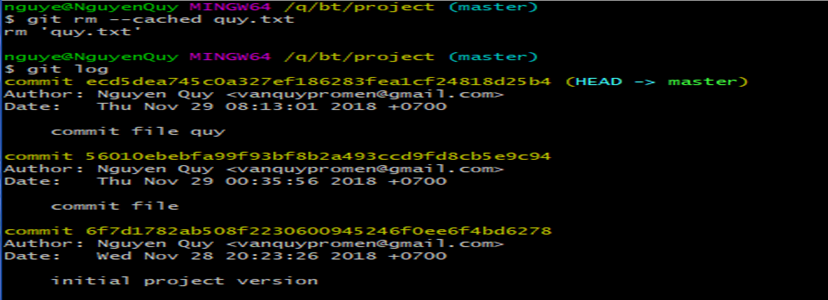
\includegraphics[width=0.8\linewidth]{screenshot017}

	\label{fig:screenshot017}
\vskip 0.4cm\vskip 0.4cm
- Ở hình trên ta thấy Git đã hiển thị tất cả các lịch sử hoạt động của user. Ví dụ: Nguyen Quy đã commit file quy.txt vào 8:13 29/11/2018\vskip 0.4cm
- Có rất nhiều tuỳ chọn khác nhau cho lệnh git log, giúp ta hiển thị thứ ta thực sự muốn\vskip 0.4cm
+ Một trong những tuỳ chọn có ích nhất là -p : hiển thị sự khác nhau của từng commit. Có thể thêm -<x> để hiển thị x commit gần nhất. VD hiển thị sự khác nhau giữa 2 commit gần nhất: {\it git log –p -2}
\vskip 0.4cm
	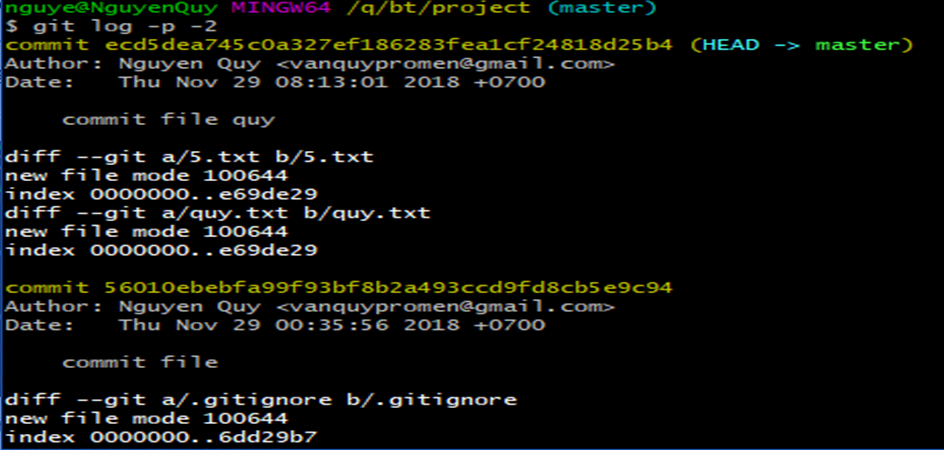
\includegraphics[width=0.8\linewidth]{screenshot018}
	
	\label{fig:screenshot018}
\vskip 0.4cm\vskip 0.4cm
+ Ở hình trên chỉ hiển thị 2 hành động gần nhất nhưng có thêm một vài thông số. Ví dụ: bạn có thể sử dụng lệnh {\it diff \texttt{-{}-}git a/5.txt b/5.txt} để so sánh sự thay đổi của tệp 5.txt (a, b ở đây chỉ phiên bản của tệp)\vskip 0.4cm

- Nếu ta muốn xem một bản thống kê tóm tắt cho mỗi commit, ta dùng lựa chọn \texttt{-{}-}stat. Lệnh {\it git log \texttt{-{}-}stat} sẽ in ra phía dưới mỗi commit danh sách các tập tin đã chỉnh sửa, bao nhiêu tập tin được sửa, và bao nhiêu dòng trong các tập tin đó được thêm vào hay xoá đi.\vskip 0.4cm

	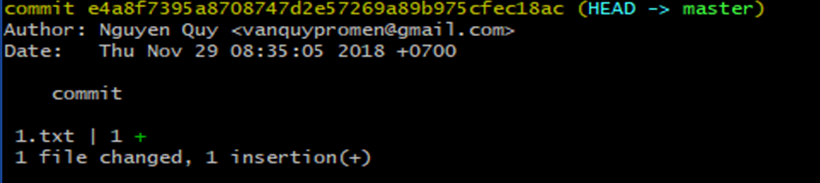
\includegraphics[width=0.8\linewidth]{screenshot019}

	\label{fig:screenshot019}
\vskip 0.4cm\vskip 0.4cm
+ Như hình trên, Git đã hiện thị vào lần commit lúc 8:35 29/11, đã có 1 tệp thay đổi và tệp đó có thêm 1 dòng\vskip 0.4cm
- Một lựa chọn hữu ích khác là \texttt{-{}-}pretty. Lựa chọn này thay đổi phần hiển thị theo các cách khác nhau.\vskip 0.4cm
+ Lựa chọn oneline in ra mỗi commit trên một dòng, thuận tiện cho việc xem nhiều commit: {\it git log \texttt{-{}-}pretty=oneline}\vskip 0.4cm

	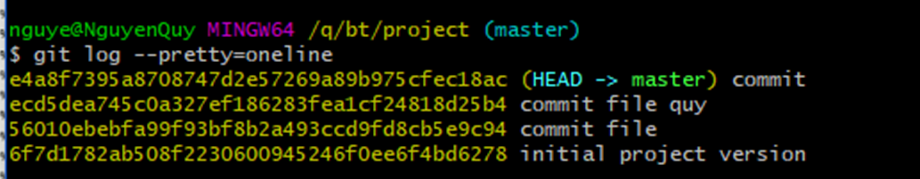
\includegraphics[width=0.8\linewidth]{screenshot020}
	
	\label{fig:screenshot020}
\vskip 0.4cm\vskip 0.4cm
+ Ta đã sử dụng {\it option \texttt{-{}-}pretty=oneline} để hiển thị mỗi commit chỉ là một dòng gồm commit ID và tin nhắn của mỗi lần commit\vskip 0.4cm
+ Lựa chọn thú vị nhất là {\it \texttt{-{}-}pretty=format}, cho phép ta chỉ định định dạng riêng của phần hiển thị.
\vskip 0.4cm
	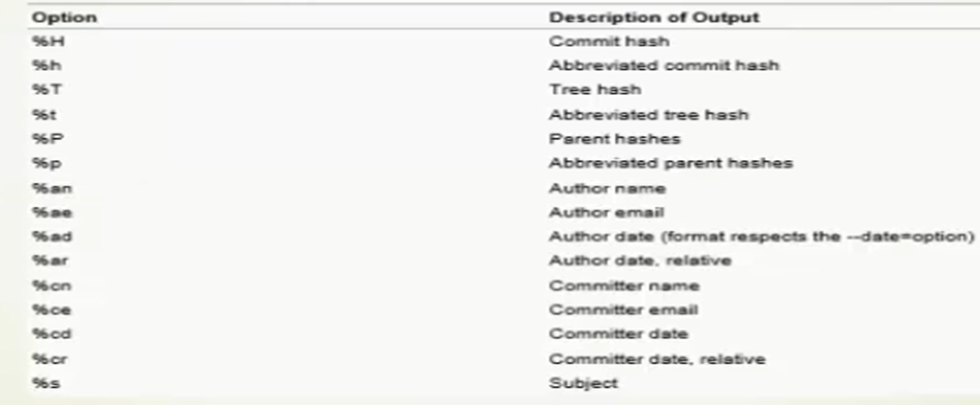
\includegraphics[width=0.8\linewidth]{screenshot021}

	\label{fig:screenshot021}
\vskip 0.4cm\vskip 0.4cm
+ Ví dụ: {\it git log \texttt{-{}-}pretty=format:”\%h - \%an, \%ar : \%s”}. Kết quả thu được\vskip 0.4cm

	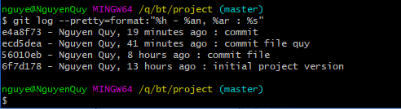
\includegraphics[width=0.8\linewidth]{screenshot022}

	\label{fig:screenshot022}
\vskip 0.4cm\vskip 0.4cm
+ Kết quả hiển thị commit ID thu gọn, tên tác giả, thời gian commit và tin nhắn cho mỗi lần commit. Với các option format này bạn có thể vận dụng cho việc báo cáo về tiến độ và kiểm soát làm việc cho từng thành viên\vskip 0.4cm
 Giới hạn thông tin đầu ra\vskip 0.4cm
- Các lựa chọn giới hạn thời gian thông tin đầu ra như \texttt{-{}-}since và \texttt{-{}-}until khá hữu ích\vskip 0.4cm

	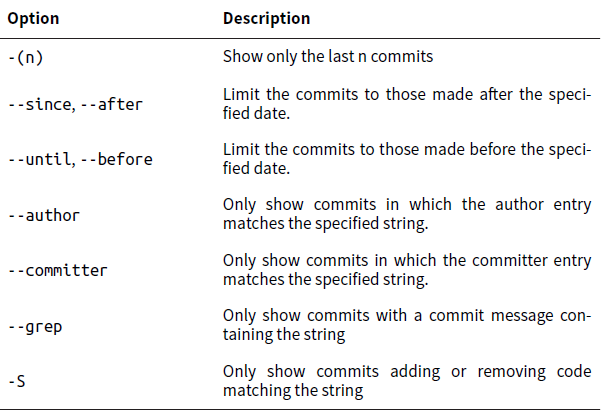
\includegraphics[width=0.8\linewidth]{screenshot023}

	\label{fig:screenshot023}
\vskip 0.4cm\vskip 0.4cm
+ Ví dụ: lệnh để hiển thị các commit từ 2 tuần trước trở lại do Nguyen Quy tạo ra:{\it git log \texttt{-{}-}pretty="\%h - \%s" \texttt{-{}-}author="Nguyen Quy" \texttt{-{}-}since=2.week }. Kết quả sẽ được:\vskip 0.4cm

	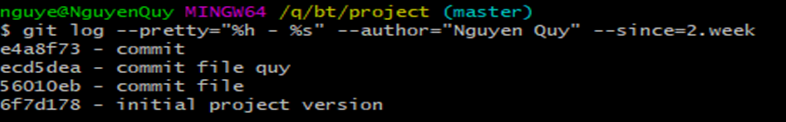
\includegraphics[width=0.8\linewidth]{screenshot024}

	\label{fig:screenshot024}
\vskip 0.4cm\vskip 0.4cm
+ Các option trên rất thích hợp cho bạn điều tra sai phạm trong dự án như là: tìm thấy người đã xóa tệp hay chỉnh sửa sai, thời gian xóa,…\vskip 0.4cm
- Ngoài ra còn 1 số option khác bạn có thể tìm hiểu thêm:
\vskip 0.4cm
	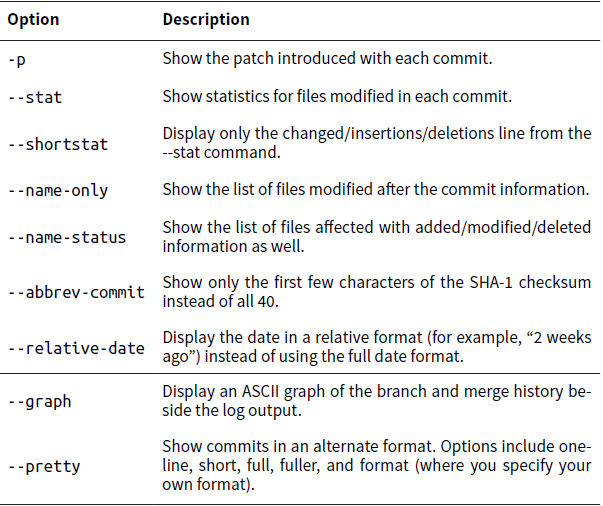
\includegraphics[width=0.8\linewidth]{screenshot025}

	\label{fig:screenshot025}




	
\section{Hủy bỏ thay đổi}
\hspace{0.6cm}{\bf a. Undoing thing} \vskip 0.4cm
- Khi bạn commit quá sớm và quên thêm các tệp khác hoặc bị lỗi phần message và muốn thử lại lần commit đó thì sử dụng:{\it git commit –amend}\vskip 0.4cm
+ Ban đầu ta chỉ có một tệp 6.txt mới được tạo và ta muốn thêm vào commit với tin nhắn là “commit 1”\vskip 0.4cm

	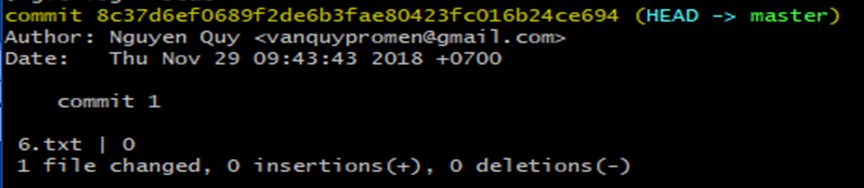
\includegraphics[width=0.8\linewidth]{screenshot026}

	\label{fig:screenshot026}
\vskip 0.4cm\vskip 0.4cm
+ Sau đó ta thêm 1 tệp 7.txt và không muốn tách ra làm 2 commit với tệp 6.txt mà muốn thêm vào “commit 1” trước đó với lệnh: {\it git commit - -amend}\vskip 0.4cm

	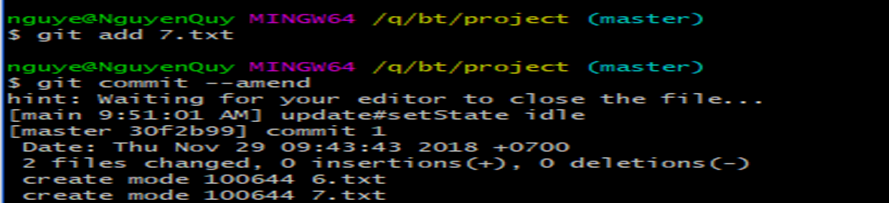
\includegraphics[width=0.8\linewidth]{screenshot027}

	\label{fig:screenshot027}
\vskip 0.4cm\vskip 0.4cm
+ Kết quả trong git log là:\vskip 0.4cm

	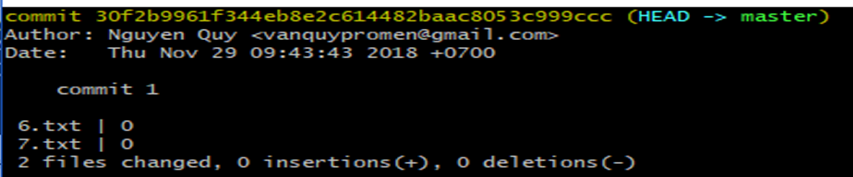
\includegraphics[width=0.8\linewidth]{screenshot028}
	
	\label{fig:screenshot028}
\vskip 0.4cm\vskip 0.4cm

{\bf b. Unstaging a staged file}\vskip 0.4cm
- Giả sử bạn đã chỉnh sửa hai tệp và muốn commit từng chỉnh sửa riêng, nhưng bạn vô tình gõ git add * và tổ chức (staged) cả hai\vskip 0.4cm
- Để unstage một tập tin:{\it git reset HEAD <name>}\vskip 0.4cm
Ví dụ: Hai tệp 1.txt và 2.txt đã được chỉnh sửa và đang ở trạng thái modified và thêm vào staged\vskip 0.4cm

	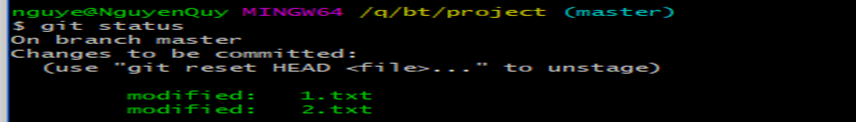
\includegraphics[width=0.8\linewidth]{screenshot029}

	\label{fig:screenshot029}
\vskip 0.4cm\vskip 0.4cm
+ Nhưng giờ bạn muốn chỉ commit tệp 1.txt ở đợt commit này thì bạn phải unstaging tệp 2.txt đã được staged bằng lệnh: {\it git reset HEAD 2.txt}. Kết quả sẽ là:\vskip 0.4cm

	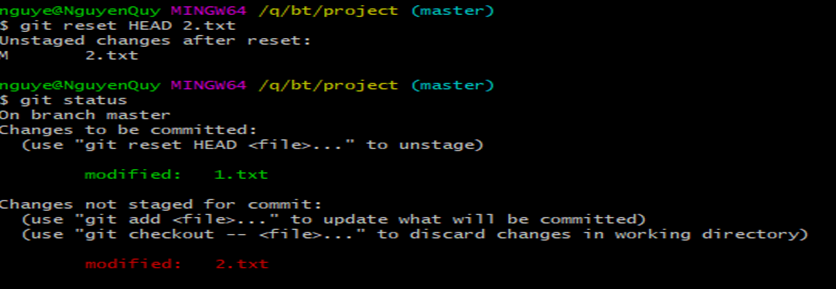
\includegraphics[width=0.8\linewidth]{screenshot030}

	\label{fig:screenshot030}
\vskip 0.4cm\vskip 0.4cm
{\bf c. Unmodifying a modified file}\vskip 0.4cm
- Trong khi bạn làm việc, sẽ có những thay đổi trên tệp mà bạn không mong muốn, bạn muốn loại bỏ đi sự thay đổi đó để quay về với nội dung cũ thì sử dụng lệnh: {\it git checkout - - <tên tệp>}\vskip 0.4cm
- Lưu ý rằng đây là một lệnh nguy hiểm – mọi thay đổi của bạn đối với tệp sẽ bị mất. Hãy chắc chắn là bạn thực sự muốn bỏ các thay đổi vừa thực hiện\vskip 0.4cm
Ví dụ: Tiếp nối ví dụ phía trên, ta đang có tệp 2.txt được chỉnh sửa, giờ bạn muốn loại bỏ đi sự thay đổi đó thì sử dụng lệnh: {\it git checkout - - 2.txt}. Kết quả thu được\vskip 0.4cm

	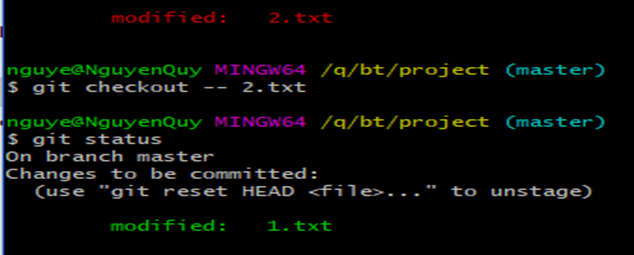
\includegraphics[width=0.8\linewidth]{screenshot031}

	\label{fig:screenshot031}
\vskip 0.4cm\vskip 0.4cm
+Tệp 2.txt đã quay trở lại trước khi thay đổi và Git thông báo không có sự thay đổi nào\vskip 0.4cm




\newpage
\section{Làm việc với remote repository}
\hspace{0.6cm}{\bf a. Tổng quan} \vskip 0.4cm
- Để có thể cộng tác trên bất kỳ dự án nào với Git, bạn cần biết cách quản lý remote repo (kho lưu trữ từ xa) của mình\vskip 0.4cm
- Remote repositories (Kho lưu trữ từ xa) là các phiên bản của dự án được lưu trữ trên Internet,  trên một máy chủ được được các tổ chức cung cấp\vskip 0.4cm
- Cộng tác với những người khác liên quan đến việc quản lý remote repo này, đẩy dữ liệu lên và kéo dữ liệu  từ chúng khi bạn cần chia sẻ công việc\vskip 0.4cm
- Quản lý remote repository bao gồm biết cách thêm, xóa các điều khiển từ xa không còn hợp lệ, quản lý các nhánh từ xa (remote branch) khác nhau và xác định chúng như đang được theo dõi hay không và hơn thế nữa\vskip 0.4cm
{\bf b. Hiển thị remotes} \vskip 0.4cm
- Để xem remote repo nào bạn đã cấu hình, bạn có thể chạy lệnh git remote\vskip 0.4cm
- Nó liệt kê các tên ngắn của mỗi remote\vskip 0.4cm
- Nếu bạn đã sao chép remote của mình, bạn nên xem nguồn gốc - đó là tên mặc định mà Git cung cấp cho máy chủ mà bạn đã sao chép từ:\vskip 0.4cm
+ git clone https://github.com/nguyenquy43/first.git\vskip 0.4cm
+ cd git\vskip 0.4cm
+ git remote: xem thông tin remote repository bạn mới lưu về máy\vskip 0.4cm

	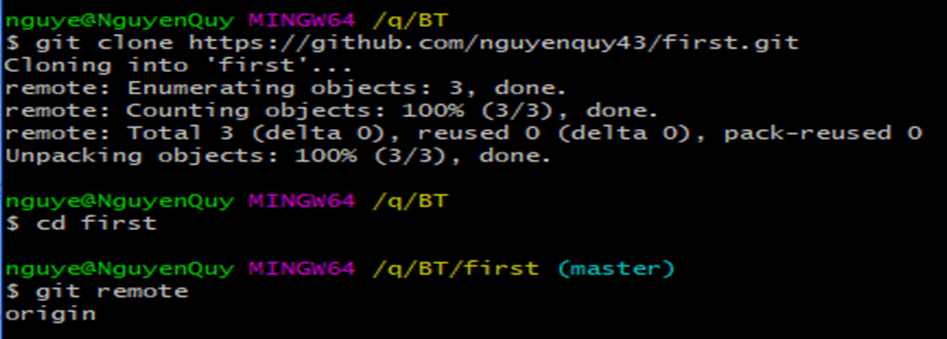
\includegraphics[width=0.8\linewidth]{screenshot032}
	
	\label{fig:screenshot032}
\vskip 0.4cm\vskip 0.4cm
- Bạn có thể dùng –v để hiển thị URL mà Git đã lưu trữ cho tên ngắn được sử dụng khi đọc và ghi vào remote đó:{\it git remote -v}\vskip 0.4cm

	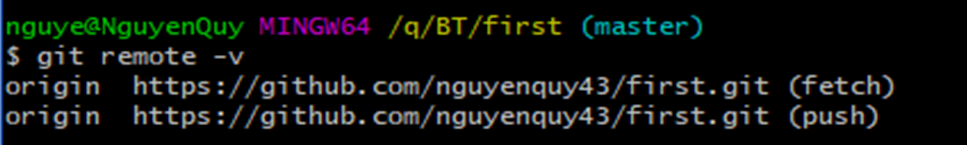
\includegraphics[width=0.8\linewidth]{screenshot033}
	
	\label{fig:screenshot033}
\vskip 0.4cm\vskip 0.4cm
+ fetch là link để ta lấy dữ liệu từ remote, push là link để ghi dữ liệu lên remote\vskip 0.4cm
{\bf c. Thêm remote repository}\vskip 0.4cm
- Khi bạn có sẵn một repository trong máy, và bạn muốn liên kết với một remote repository\vskip 0.4cm
- Để thêm một remote repo mới dưới dạng một tên ngắn:{\it git remote add <shortname> <url>}\vskip 0.4cm
- Ví dụ: 
\vskip 0.4cm
	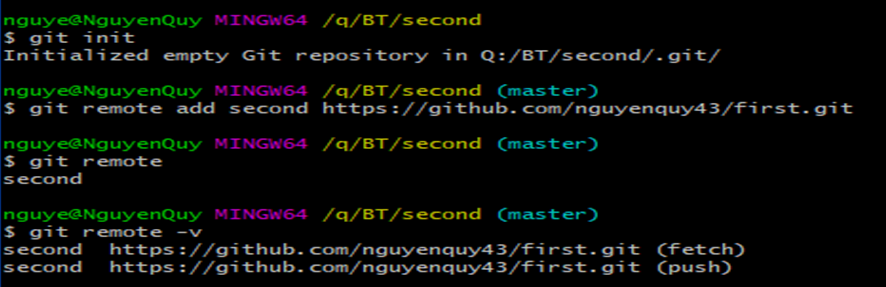
\includegraphics[width=0.8\linewidth]{screenshot034}
	
	\label{fig:screenshot034}
\vskip 0.4cm\vskip 0.4cm
{\bf d. Nạp và kéo dữ liệu từ remote repository} \vskip 0.4cm
- Lệnh đi đến remote repo và kéo tất cả dữ liệu từ remote repo mà bạn chưa có:{\it git fetch <remote name>}\vskip 0.4cm
- Điều cần lưu ý là lệnh git fetch chỉ tải dữ liệu xuống  local repo của bạn - nó không tự động kết hợp (merge) dữ liệu đó với bất kỳ dữ liệu nào của bạn hoặc sửa đổi những gì bạn hiện đang làm việc\vskip 0.4cm
- Bạn có thể sử dụng lệnh git pull để tự động tìm nạp và sau đó hợp nhất nhánh từ xa (remote branch) đó vào nhánh hiện tại của bạn:{\it git pull <remote name> <branch name>}\vskip 0.4cm
- Ví dụ: \vskip 0.4cm

	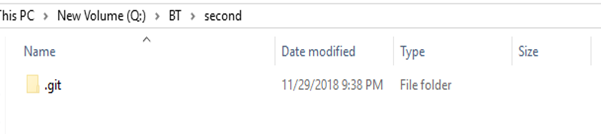
\includegraphics[width=0.8\linewidth]{screenshot035}

	\label{fig:screenshot035}

\vskip 0.4cm\vskip 0.4cm
	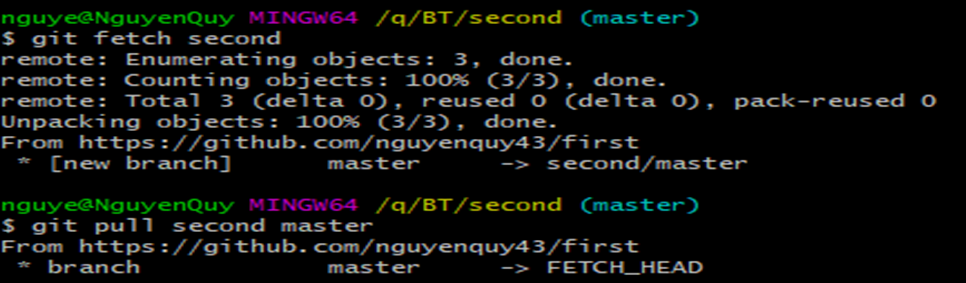
\includegraphics[width=0.8\linewidth]{screenshot036}

	\label{fig:screenshot036}
\vskip 0.4cm\vskip 0.4cm
+ Kết quả thu được là: \vskip 0.4cm

	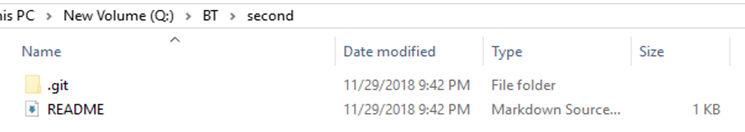
\includegraphics[width=0.8\linewidth]{screenshot037}

	\label{fig:screenshot037}
\vskip 0.4cm\vskip 0.4cm
+ Tệp README đã được kéo về từ kho lữu trữ về second remote repository\vskip 0.4cm
{\bf e. Đẩy lên remote repo} \vskip 0.4cm
- Khi bạn có một điểm trong dự án mà bạn muốn chia sẻ, bạn phải đẩy (pushing) bằng lệnh: {\it git push <remote name> <brach name> }\vskip 0.4cm
- Lệnh này chỉ hoạt động nếu bạn nhân bản (clone) từ một máy chủ mà bạn có quyền truy cập ghi và không có ai đẩy trong thời gian đó\vskip 0.4cm
- Ví dụ: Trong project second ta đã thêm một tệp text.txt và bây giờ ta cần thêm nó vào local repository và đưa nó lên kho dữ liệu\vskip 0.4cm

	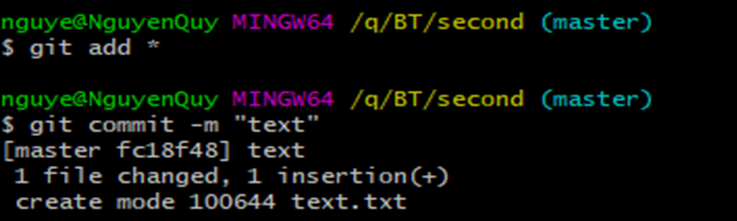
\includegraphics[width=0.8\linewidth]{screenshot038}

	\label{fig:screenshot038}
\vskip 0.4cm\vskip 0.4cm
+ Sau khi đã commit, ta tiến hành đưa lên remote repository bằng lệnh: git push second master
\vskip 0.4cm

	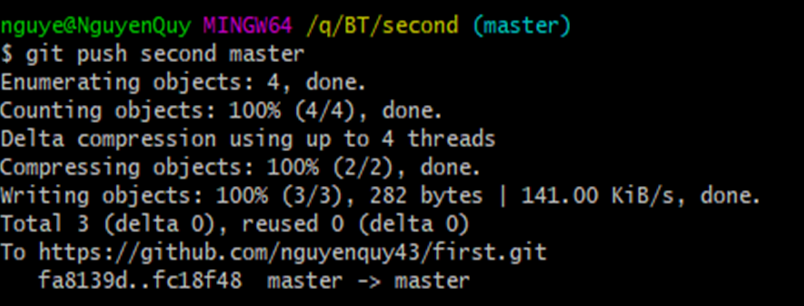
\includegraphics[width=0.8\linewidth]{screenshot039}

	\label{fig:screenshot039}
\vskip 0.4cm\vskip 0.4cm
{\bf f. Kiểm tra remote} \vskip 0.4cm
- Nếu bạn muốn xem thêm thông tin về một remote cụ thể:{\it git remote show <remote name>}\vskip 0.4cm


	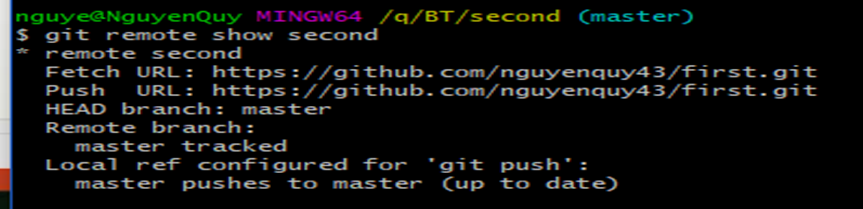
\includegraphics[width=0.8\linewidth]{screenshot040}

	\label{fig:screenshot040}\vskip 0.4cm\vskip 0.4cm

{\bf g. Xóa và đổi tên remotes} \vskip 0.4cm
- Bạn thay đổi shortname của remote:{\it git remote rename <tên remote cũ> <new remote name>}\vskip 0.4cm
- Nếu muốn loại bỏ remote repo  bạn có thể sử dụng:{\it git remote rm <remote name> }
\vskip 0.4cm

	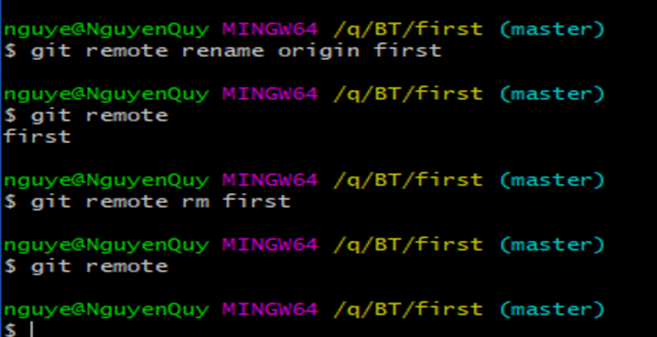
\includegraphics[width=0.8\linewidth]{screenshot041}

	\label{fig:screenshot041}
\newpage

			
\section{Làm việc với tag (thẻ) trong GIT}
\hspace{0.6cm}{\bf a. Gắn thẻ} \vskip 0.4cm
- Như hầu hết các VCS, Git có khả năng gắn thẻ (tag) các điểm cụ thể quan trọng trong quá trình phát triển\vskip 0.4cm
- Thông thường người sử dụng chức năng này dùng để các release point (đánh dấu những phiên bản và sau đó chỉ cần liệt kê theo tag đã đánh dấu để tìm những phiên bản đã được đánh dấu từ trước)\vskip 0.4cm
{\bf b. Liệt kê thẻ} \vskip 0.4cm
- Liệt kê tất cả các thẻ của bạn: git tag\vskip 0.4cm
- Bạn có thể tìm kiếm các thẻ theo một yêu cầu nhất định. Ví dụ, Git source repo chứa hơn 500 tags. Nếu bạn chỉ cần xem các thẻ có đầu là v.1.8.5git tag –l “v.1.8.5*”\vskip 0.4cm
{\bf c. Tạo thẻ} \vskip 0.4cm
- Git sử dụng hai loại thẻ chính: lightweight và annotated\vskip 0.4cm
- Một thẻ lightweight (thẻ nhẹ) nó chỉ trỏ đến một commit cụ thể:{\it git tag <tag name>-lw.} \vskip 0.4cm
	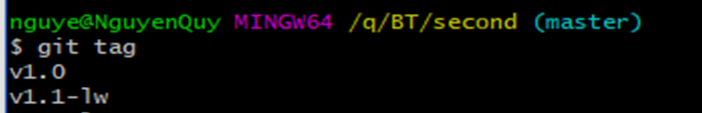
\includegraphics[width=0.8\linewidth]{screenshot042}

	\label{fig:screenshot042}
\vskip 0.4cm\vskip 0.4cm
- Thẻ annotated (thẻ lưu trữ) được lưu trữ dưới dạng các đối tượng đầy đủ trong Git:{\it git tag –a <tag name> -m “message”}. Bạn có thể xem dữ liệu thẻ cùng với commit đã được gắn thẻ bằng cách sử dụng:{\it git show <tag name>}\vskip 0.4cm

	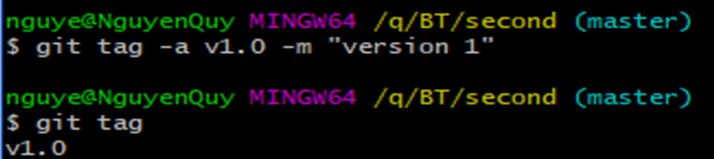
\includegraphics[width=0.8\linewidth]{screenshot043}

	\label{fig:screenshot043}\vskip 0.4cm\vskip 0.4cm

- Bạn nên thường xuyên gắn thẻ có chú thích (annotted tag) để bạn có thể có tất cả thông tin này; nhưng nếu bạn muốn một thẻ tạm thời hoặc vì một lý do nào đó không muốn giữ thông tin khác hãy sử dụng thẻ lightweight\vskip 0.4cm
{\bf d. Tagging later} \vskip 0.4cm
- Bạn cũng có thẻ gắn thẻ các commit sau khi bạn đã di chuyển chúng. Để gắn thẻ commit đó: \vskip 0.4cm
+{\it git log - -pretty=oneline}: Lệnh này để xem lịch sử các commit ở dạng một dòng, dùng để lấy checksum ID của commit\vskip 0.4cm
+ Sau đó thì thì sử dụng lệnh: {\it git tag  <tag name> <checksum ID>}\vskip 0.4cm
Ví dụ: 
\vskip 0.4cm
	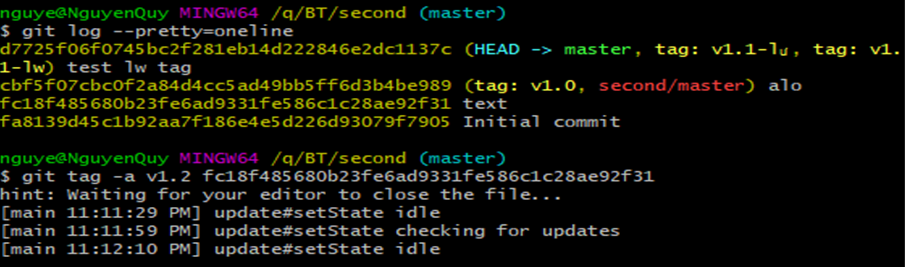
\includegraphics[width=0.8\linewidth]{screenshot044}

	\label{fig:screenshot044}
\vskip 0.4cm\vskip 0.4cm
{\bf e. Chia sẻ thẻ} \vskip 0.4cm
- Lệnh git push không thể chuyển thẻ tới máy chủ\vskip 0.4cm
- Bạn sẽ phải đẩy thẻ bằng một cách khác vào máy chủ với lệnh: {\it git push <remote name> <tag name>}\vskip 0.4cm
- Nếu bạn có nhiều thẻ mà bạn muốn đẩy lên cùng một lúc:{\it git push <remote name> - -tags}\vskip 0.4cm
- Ví dụ:\vskip 0.4cm

	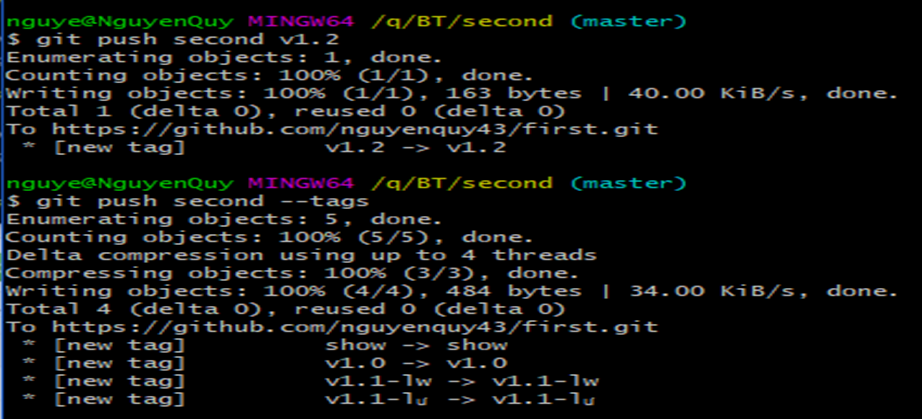
\includegraphics[width=0.8\linewidth]{screenshot045}

	\label{fig:screenshot045}
\vskip 0.4cm\vskip 0.4cm
{\bf f. Checking out tags} \vskip 0.4cm
- Bạn không thể thực sự kiểm tra thẻ trong Git, vì chúng không thể di chuyển được. Nếu bạn muốn đặt một phiên bản của kho lưu trữ trong thư mục làm việc của bạn trông giống như một thẻ cụ thể, bạn có thể tạo một chi nhánh mới tại một thẻ cụ thể với :{\it git checkout –b <branchname> <tagname>}\vskip 0.4cm
- Ví dụ: Ta có thể tạo mới một nhánh riêng có tag v1.2\vskip 0.4cm

	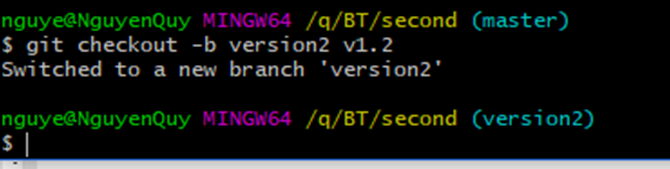
\includegraphics[width=0.8\linewidth]{screenshot046}

	\label{fig:screenshot046}
\vskip 0.4cm\vskip 0.4cm
{\bf g. Xóa thẻ}\vskip 0.4cm
- Xóa thẻ ở kho dữ liệu trên máy bạn (local repo):{\it  git tag –d <tag name>}\vskip 0.4cm
- Xóa thẻ trên máy chủ lưu trữ:{\it git push <remote name> - -delete <tag name>}\vskip 0.4cm

	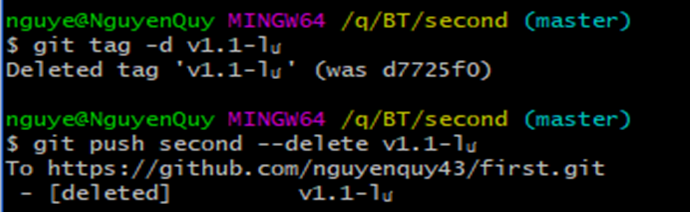
\includegraphics[width=0.8\linewidth]{screenshot047}
	
	\label{fig:screenshot047}




				
\section{Phân nhánh (branching)}
\hspace{0.6cm}- Phân nhánh nghĩa là bạn tách khỏi dòng phát triển chính của dự án và tiếp tục làm việc mà không gây rối tới dòng chính đó (dùng để phát triển tính năng cho các phần mềm không gây ảnh hưởng)\vskip 0.4cm
- Hiểu và nắm vững tính năng này cung cấp cho bạn một công cụ mạnh mẽ và độc đáo, hoàn toàn có thể thay đổi cách bạn phát triển các dự án\vskip 0.4cm
- Một ủy thác (commit) và cây của nó (trees)\vskip 0.4cm

	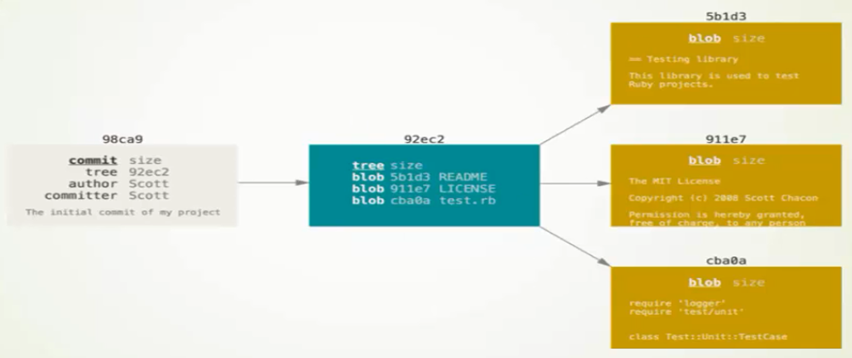
\includegraphics[width=0.8\linewidth]{screenshot048}

	\label{fig:screenshot048}
\vskip 0.4cm\vskip 0.4cm
- Nếu bạn thực hiện một số thay đổi và ủy thác một lần nữa, commit tiếp theo sẽ lưu trữ một con trỏ đến commit xuất hiện ngay trước nó\vskip 0.4cm


	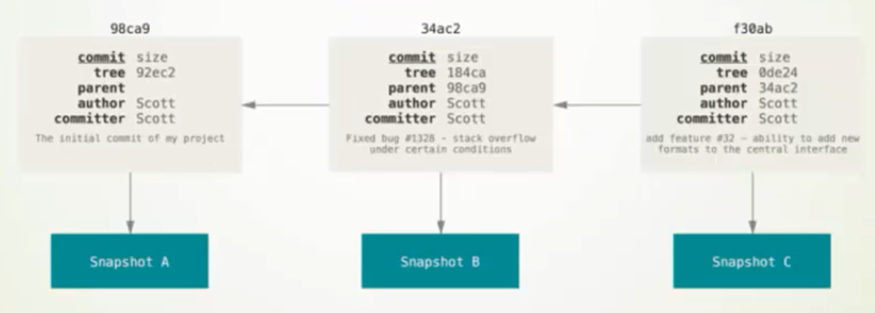
\includegraphics[width=0.8\linewidth]{screenshot049}
	
	\label{fig:screenshot049}
\vskip 0.4cm\vskip 0.4cm
- Một nhánh (branch) và lịch sử commit 	
\vskip 0.4cm
	\includegraphics[width=0.8\linewidth]{screenshot050}

	\label{fig:screenshot050}
\vskip 0.4cm\vskip 0.4cm
{\bf a. Tạo một nhánh mới}\vskip 0.4cm
- Tạo một nhánh mới bằng lệnh: {\it git branch <branch name>}\vskip 0.4cm
- Ví dụ: tạo một branch có tên là testing: git branch testing. Điều này tạo ra một con trỏ mới cho cùng một commit mà bạn đang thực hiện
\vskip 0.4cm
	\includegraphics[width=0.8\linewidth]{screenshot051}

	\label{fig:screenshot051}
\vskip 0.4cm\vskip 0.4cm
{\bf b. Con trỏ HEAD đến nhánh}\vskip 0.4cm
- Làm thế nào để Git biết bạn hiện đang thao tác ở nhánh nào? Nó được biểu diễn bằng một con trỏ đặc biệt: HEAD\vskip 0.4cm
- Bạn có thể thấy được HEAD đang trỏ tới nhánh nào bằng lệnh: {\it git log - -oneline - -decorate}\vskip 0.4cm

	\includegraphics[width=0.8\linewidth]{screenshot052}
	
	\label{fig:screenshot052}
\vskip 0.4cm\vskip 0.4cm
- Ví dụ
\vskip 0.4cm
	\includegraphics[width=0.8\linewidth]{screenshot053}
	
	\label{fig:screenshot053}
\vskip 0.4cm\vskip 0.4cm
- Chuyển nhánh để di chuyển HEAD trỏ vào nhánh được chỉ định:{\it git checkout <branch name>} \vskip 0.4cm
- Ví dụ: git checkout testing -> chuyển HEAD trỏ sang nhánh testing\vskip 0.4cm

	\includegraphics[width=0.8\linewidth]{screenshot054}

	\label{fig:screenshot054}
\vskip 0.4cm\vskip 0.4cm
{\bf c. Quản lý nhánh (Branches management)}\vskip 0.4cm
- Bạn có thể nhận được một danh sách nhánh hiện tại bằng lệnh:{\it git branch}\vskip 0.4cm

	\includegraphics[width=0.8\linewidth]{screenshot055}
	
	\label{fig:screenshot055}
\vskip 0.4cm\vskip 0.4cm
- Lưu ý ký tự * đứng trước nhánh master: nó chỉ ra nhánh mà bạn hiện đã thao tác (nhánh mà HEAD trỏ tới)\vskip 0.4cm
- Để xem lần commit cuối cùng trên mỗi nhánh:{\it git branch –v}\vskip 0.4cm
- Các tùy chọn - -merged và - -no-merged có thể lọc danh sách gồm các nhánh đã hoặc chưa được kết hợp (merge) vào nhánh hiện đang truy cập:{\it git branch - -merged} và{\it git branch - -no-merged}\vskip 0.4cm

	\includegraphics[width=0.8\linewidth]{screenshot056}

	\label{fig:screenshot056}
\vskip 0.4cm\vskip 0.4cm
- Nếu bạn thật sự muốn xóa một nhánh và công việc đang thực hiện trên nhánh đó thì có thể sử dụng lệnh: {\it git branch –D <branch name>}\vskip 0.4cm

	\includegraphics[width=0.8\linewidth]{screenshot057}

	\label{fig:screenshot057}
\vskip 0.4cm\vskip 0.4cm
{\bf d. Phân nhánh luồng công việc}\vskip 0.4cm
- Long-running branches (nhánh dài hạn): là các nhánh chính, đi xuyên suốt trong quá trình phát triển dự án\vskip 0.4cm
+ Vì Git sử dụng một three-way merge đơn giản (là kết hợp 3 lần commit), việc hợp nhất từ nhánh này sang nhánh khác trong thời gian khác rất dễ thực hiện\vskip 0.4cm
+ Điều này có nghĩa là bạn có thể có nhiều nhánh luôn mở và bạn sử dụng cho các giai đoạn khác nhau trong chu kỳ phát triển dự án; bạn có thể thường xuyên merge (kêt hợp) từ một số nhánh trong số đó thành nhánh khác
\vskip 0.4cm
	\includegraphics[width=0.8\linewidth]{screenshot058}

	\label{fig:screenshot058}
\vskip 0.4cm\vskip 0.4cm
- Topic branches (nhánh ngắn hạn): các nhánh thường được tạo ra với mục đích sửa lỗi, sau khi sửa lỗi không mà được merge với nhánh chính thì sẽ bị xóa\vskip 0.4cm

						\includegraphics[width=0.8\linewidth]{screenshot059}
					
						\label{fig:screenshot059}
				\vskip 0.4cm\vskip 0.4cm
					* Quan trọng: Khi bạn đang branching (phân nhánh) và kết hợp (merging), mọi thứ chỉ được thực hiện trong kho lưu trữ Git của bạn (local repo) - không có giao tiếp với máy chủ nào đang diễn ra\vskip 0.4cm
					
					
					\newpage
\section{Hợp (merge) nhánh và xử lý xung đột (conlicts)}
\hspace{0.6cm}- Merge branch tức là bạn gộp hai branch lại với nhau, thao tác này thường dùng để merge branch khác vào branch master trước khi push lên remote repository, hoặc merge hai branch thành một để giải quyết chung một task.	\vskip 0.4cm
{\bf a. Basic merging}	\vskip 0.4cm
- Hãy tích hợp thay đổi đã thực hiện trên branch issue1 vào branch master	\vskip 0.4cm

	\includegraphics[width=0.8\linewidth]{screenshot060}

	\label{fig:screenshot060}	\vskip 0.4cm	\vskip 0.4cm

- Merge 2 nhánh sẽ được thực hiện bằng lệnh merge:{\it git merge <branch name>.}	\vskip 0.4cm 
- Đầu tiên, sử dụng lệnh git checkout master để chuyển con trỏ HEAD đến nhánh master	\vskip 0.4cm

	\includegraphics[width=0.8\linewidth]{screenshot061}

	\label{fig:screenshot061}
	\vskip 0.4cm	\vskip 0.4cm
- Tệp được chỉnh sửa là tệp issue.txt có nội dung:{\it ''  Đây là nội dung gốc ''}	\vskip 0.4cm
- Chỉnh sửa tệp issue.txt trong branch issue1:{\it '' Đây là nội dung chỉnh sửa ''}	\vskip 0.4cm
- Ta thực hiện tích hợp sự thay đổi trong tệp issue.txt giữa 2 nhánh	\vskip 0.4cm

	\includegraphics[width=0.8\linewidth]{screenshot062}

	\label{fig:screenshot062}
	\vskip 0.4cm	\vskip 0.4cm
- Nội dung của tệp issue.txt sau merge:	\vskip 0.4cm
\hspace{1cm}{\it''Đây là nội dung gốc}	\vskip 0.1cm
\hspace{1cm}{\it Đây là nội dung chỉnh sửa''}	\vskip 0.4cm
{\bf b. Basic merge conflicts}	\vskip 0.4cm
- Giả sử, có 2 người đang cùng sửa 1 lỗi trên tệp issue.txt tại 2 branch khác nhau là issue2 và issue3	\vskip 0.4cm
- Bây giờ, hãy tích hợp thay đổi tại branch issue2 và thay đổi tại branch issue3 vào master.	\vskip 0.4cm
- Trước tiên, sau khi đã checkout trên branch master, thực hiện merge branch issue2.	\vskip 0.4cm
{\it \hspace{1cm}\$ git checkout master	\vskip 0.1cm
\hspace{1cm}Switched to branch 'master'	\vskip 0.1cm
\hspace{1cm}\$ git merge issue2	\vskip 0.1cm
\hspace{1cm}Updating b2b23c4..8f7aa27	\vskip 0.1cm
\hspace{1cm}Fast-forward	\vskip 0.1cm
\hspace{1cm}issue.txt |    2 ++	\vskip 0.1cm
\hspace{1cm}1 files changed, 2 insertions(+), 0 deletions(-)}	\vskip 0.4cm

- Như vậy merge fast-forward (chuyển tiếp nhanh) sẽ được thực hiện.	\vskip 0.4cm

	\includegraphics[width=0.8\linewidth]{screenshot063}

	\label{fig:screenshot063}
	\vskip 0.4cm	\vskip 0.4cm
- Tiếp theo, thực hiện merge branch issue3.	\vskip 0.4cm
{\it \hspace{1cm}\$ git merge issue3	\vskip 0.1cm
\hspace{1cm}Auto-merging issue.txt	\vskip 0.1cm
\hspace{1cm}CONFLICT (content): Merge conflict in issue.txt	\vskip 0.1cm
\hspace{1cm}Automatic merge failed; fix conflicts and then commit the result.}	\vskip 0.4cm

- Tự động merge đã thất bại. Có vẻ như đã phát sinh xung đột do đã thay đổi cùng một dòng với nội dung khác. Nội dung của issue.txt lúc này thì sẽ giống như bên dưới.	\vskip 0.4cm
{\it \hspace{1cm}Đây là nội dung gốc	\vskip 0.1cm
\hspace{1cm}Đây là nội dung chỉnh sửa	\vskip 0.1cm
\hspace{1cm}<<<<<<< HEAD	\vskip 0.1cm
\hspace{1cm}commit: Đây là nội dung chỉnh sửa issue2	\vskip 0.1cm
\hspace{1cm}=======	\vskip 0.1cm
\hspace{1cm}pull: Đây là nội dung chỉnh sửa issue3	\vskip 0.1cm
\hspace{1cm}>>>>>>> issue3}	\vskip 0.4cm
- Ở những chổ có xung đột thì Git đang chèn vào phần khác biệt. Hãy sửa như bên dưới.	\vskip 0.4cm
{\it \hspace{1cm}Đây là nội dung gốc	\vskip 0.1cm
\hspace{1cm}Đây là nội dung chỉnh sửa	\vskip 0.1cm
\hspace{1cm}commit: Đây là nội dung chỉnh sửa issue2	\vskip 0.1cm
\hspace{1cm}pull: Đây là nội dung chỉnh sửa issue3}	\vskip 0.4cm
- Vì đã chỉnh sửa nơi xung đột nên hãy commit lại.	\vskip 0.4cm
{\it \hspace{1cm}\$ git add issue.txt	\vskip 0.1cm
\hspace{1cm}\$ git commit -m "Thực hiện merge branch issue3"	\vskip 0.1cm \hspace{1cm}
\hspace{1cm}\# On branch master	\vskip 0.1cm
\hspace{1cm}nothing to commit (working directory clean)}	\vskip 0.4cm
- Lịch sử sẽ giống thế này. Vì đã chỉnh sửa nơi xung đột trong merge lần này, nên merge commit sẽ ghi lại thay đổi đó sẽ được tạo mới. Và, đầu của master sẽ di chuyển đến đó. Loại merge thế này là không phải fast-forward mà được gọi là non fast-forward merge.
	\vskip 0.4cm
	\includegraphics[width=0.8\linewidth]{screenshot064}

	\label{fig:screenshot064}

	\vskip 0.4cm	\vskip 0.4cm
			\newpage			
\section{Remote branches}
\hspace{0.6cm}- Tại đường dẫn {\it /q/BT/example/remote} tạo một remote repo trên máy local bằng lệnh{\it git init - -bare} \vskip 0.4cm
- Ta có một local repo tên local với snapshot như hình\vskip 0.4cm

	\includegraphics[width=0.8\linewidth]{screenshot065}
	
	\label{fig:screenshot065}\vskip 0.4cm\vskip 0.4cm

- Tiến hành thiết lập remote cho nó bằng lệnh: {\it git remote add <remote  name> <address>} đặt tên remote là origin với địa chỉ là{\it /q/BT/example/remote}\vskip 0.4cm

	\includegraphics[width=0.8\linewidth]{screenshot066}

	\label{fig:screenshot066}
\vskip 0.4cm\vskip 0.4cm
- Tiến hành push tất cả dữ liệu từ repo local lên remote repo:{\it git push - -all origin}
\vskip 0.4cm
{\it  \hspace{1cm}\$ git remote add origin /q/BT/example/remote\vskip 0.1cm
 \hspace{1cm}To Q:/BT/example/remote\vskip 0.1cm
 \hspace{1cm}* [new branch]      alpha -> alpha\vskip 0.1cm
 \hspace{1cm}* [new branch]      master -> master}\vskip 0.4cm

 - Clone (nhân bản) từ remote repo:{\it git clone <address remote repo> <address clone>}\vskip 0.4cm
 
 {\it \hspace{1cm} \$ git clone /q/BT/example/remote /q/BT/example/clone\vskip 0.1cm
 \hspace{1cm} Cloning into 'Q:/BT/example/clone'...\vskip 0.1cm
 \hspace{1cm} done.}\vskip 0.4cm
 
 - Các ví dụ sẽ được lấy từ repo clone\vskip 0.4cm
 - Trong một Local Repo, nếu Remote đặt tên là remotename, và một nhánh tên là branchname thì để biểu thị nhánh này trên Remote sẽ ký hiệu là remotename/branchename. Trạng thái sau khi nhân bản (clone)\vskip 0.4cm
 {\bf a. Trạng thái của của remote và clone}\vskip 0.4cm
 - Kiểm tra trạng thái của repo clone\vskip 0.4cm

 	\includegraphics[width=0.8\linewidth]{screenshot067}
 
 	\label{fig:screenshot067}
\vskip 0.4cm\vskip 0.4cm
 - Trạng thái của remote:\vskip 0.4cm

 	\includegraphics[width=0.8\linewidth]{screenshot068}

 	\label{fig:screenshot068}
\vskip 0.4cm\vskip 0.4cm
 - Nhánh master của cả 2 đều đang ở snapshot C2\vskip 0.4cm
{\bf b. Sự phân nhánh tại Local khi Remote cập nhật:}\vskip 0.4cm
 - Giả sử ở repo local, có thêm 2 commit mới là snapshot C3, C4, sau đó cập nhật nhánh master lên remote:{\it git push origin master}\vskip 0.4cm


 	\includegraphics[width=0.8\linewidth]{screenshot069}

 	\label{fig:screenshot069}
\vskip 0.4cm\vskip 0.4cm
 	\includegraphics[width=0.8\linewidth]{screenshot070}
 
 	\label{fig:screenshot070}\vskip 0.4cm\vskip 0.4cm

 - Quay lại với repo clone, ta cũng tạo 2 commit C5, C6 nhưng không đẩy lên remote: ta thấy nhánh master \vskip 0.4cm
 
 	\includegraphics[width=0.8\linewidth]{screenshot071}
 
 	\label{fig:screenshot071}
 \vskip 0.4cm\vskip 0.4cm
 	\includegraphics[width=0.8\linewidth]{screenshot072}
 
 	\label{fig:screenshot072}
\vskip 0.4cm\vskip 0.4cm
 - Tiếp theo, sử dụng lệnh{\it git fetch --all} để  tìm trong origin những dữ liệu mới sau đó cập nhật dữ liệu vào repo clone và kiểm tra trạng thái\vskip 0.4cm

 	\includegraphics[width=0.8\linewidth]{screenshot073}
 
 	\label{fig:screenshot073}\vskip 0.4cm\vskip 0.4cm

 - Nó cho biết nhánh master và origin/master tại repo colne bị phân nhánh. Có thể chuyển xem log của origin/master
\vskip 0.4cm
 	\includegraphics[width=0.8\linewidth]{screenshot074}
 
 	\label{fig:screenshot074}
 \vskip 0.4cm\vskip 0.4cm
 - Qua đó dựng được tình trạng master và origin/master bị phân ly ở repo clone như sau:\vskip 0.4cm

 	\includegraphics[width=0.8\linewidth]{screenshot075}
 
 	\label{fig:screenshot075}
 \vskip 0.4cm\vskip 0.4cm
{\bf c. Pull – Hợp nhánh bị phân ly}\vskip 0.4cm
 - Để hợp nhánh phân ly trên dùng lệnh merge để hợp nhánh origin/master vào master sau khi fetch dữ liệu về\vskip 0.4cm
 - Quá trình trên có thể tự động luôn cả 2 (tức là fetch xong, merge luôn) bằng lệnh git pull origin master\vskip 0.4cm
 -  Sau khi pull kiểm tra log:\vskip 0.4cm
 
 \includegraphics[width=0.8\linewidth]{screenshot076}
 	\label{fig:screenshot076}
\vskip 0.4cm\vskip 0.4cm
 	\includegraphics[width=0.8\linewidth]{screenshot077}

 	\label{fig:screenshot077}
\vskip 0.4cm\vskip 0.4cm
 - Xóa nhánh tại remote
 \vskip 0.4cm
 {\it \hspace{1cm} \$ git push remotename --delete branchname}\vskip 0.4cm
 
 - Đổi tên nhánh local và remote\vskip 0.4cm
 
 {\it \hspace{1cm}git branch -m old\_branch new\_branch         \hspace{1cm} \# Đổi tên ở Local\vskip 0.1cm
  \hspace{1cm}git push origin :old\_branch                  \hspace{1cm}\# Xóa nhánh ở Remote\vskip 0.1cm
  \hspace{1cm}git push --set-upstream origin new\_branch   \# Cập nhật nhánh có tên mới lên  Remote\vskip 0.4cm }

 - Cập nhật nhánh mới từ remote vào local\vskip 0.4cm
 
 {\it \hspace{1cm}git pull origin                                    \hspace{1cm}\# Cập nhật thông tin từ Remote\vskip 0.1cm
  \hspace{1cm}git branch -r                                      \hspace{1cm}\# Liệt kê các nhánh ở Remote\vskip 0.1cm
  \hspace{1cm}git checkout -b branchname  origin/branchname      \hspace{1cm}\# Tao nhánh mới ở Local theo Remote\vskip 0.4cm}
 
							
\section{Rebasing}
\hspace{0.6cm}- Khái niệm: Lệnh này sẽ merge hai branch lại với nhau và nó sẽ chọn commit mới nhất (snapshot mới nhất) để thực hiện. Nhưng với rebase thì cơ chế hoạt động có chút khác biệt, nó sẽ so sánh và lưu những thay đổi giữa hai nhánh vào một file tạm, sau đó thực hiện fast-forward merge
\newpage

\chapter{Tổng kết} % Chương 3
\hspace{0.6cm} Trên đây  là toàn bộ kiến thức mà nhóm đã học được trong thời gian tìm hiểu về GIT, qua đó nhóm đã thấy được nhưng lợi ích của GIT trong quá trình học tập và làm việc, đặc biệt là trong quá trình làm việc nhóm hay giải quyết những dự án lớn:\vskip 0.4cm
-Sắp xếp công việc tốt hơn\vskip 0.4cm
-Linh hoạt hơn khi cùng phải làm cùng lúc nhiều task\vskip 0.4cm
-Tự tin hơn khi thử nghiệm những ý tưởng mới \vskip 0.4cm
-GitHub Community Forum là nơi để lập trình viên trao đổi, hỗ trợ và học hỏi với hơn 439000 developers và 1 triệu 350 ngàn repositories, đây chính là nơi hỗ trợ cho những bạn mới bắt đầu với git.\vskip 0.4cm
...\vskip 0.4cm

\begin{thebibliography}{99} % Tài liệu tham khảo

%\addcontentsline{toc}{chapter}{{\bf Tài liệu tham khảo}\rm}

\bibitem{Eva} Sách {\it Pro Git} của tác giả Scott Chacon và Ben Straub

\bibitem{BaI} Các nguồn tài liệu trên mạng và youtube.

% Chú thích: mỗi tài liệu là một bibitem.

\end{thebibliography}

\end{document}